\documentclass{standalone}
\usepackage{tikz}
\usetikzlibrary{patterns}
\usetikzlibrary{positioning}
\usetikzlibrary{patterns, positioning}
\usetikzlibrary{shapes.misc}
\usepackage[outline]{contour}
\contourlength{1.5pt} 
\usepackage[sfdefault]{ClearSans}

\begin{document}
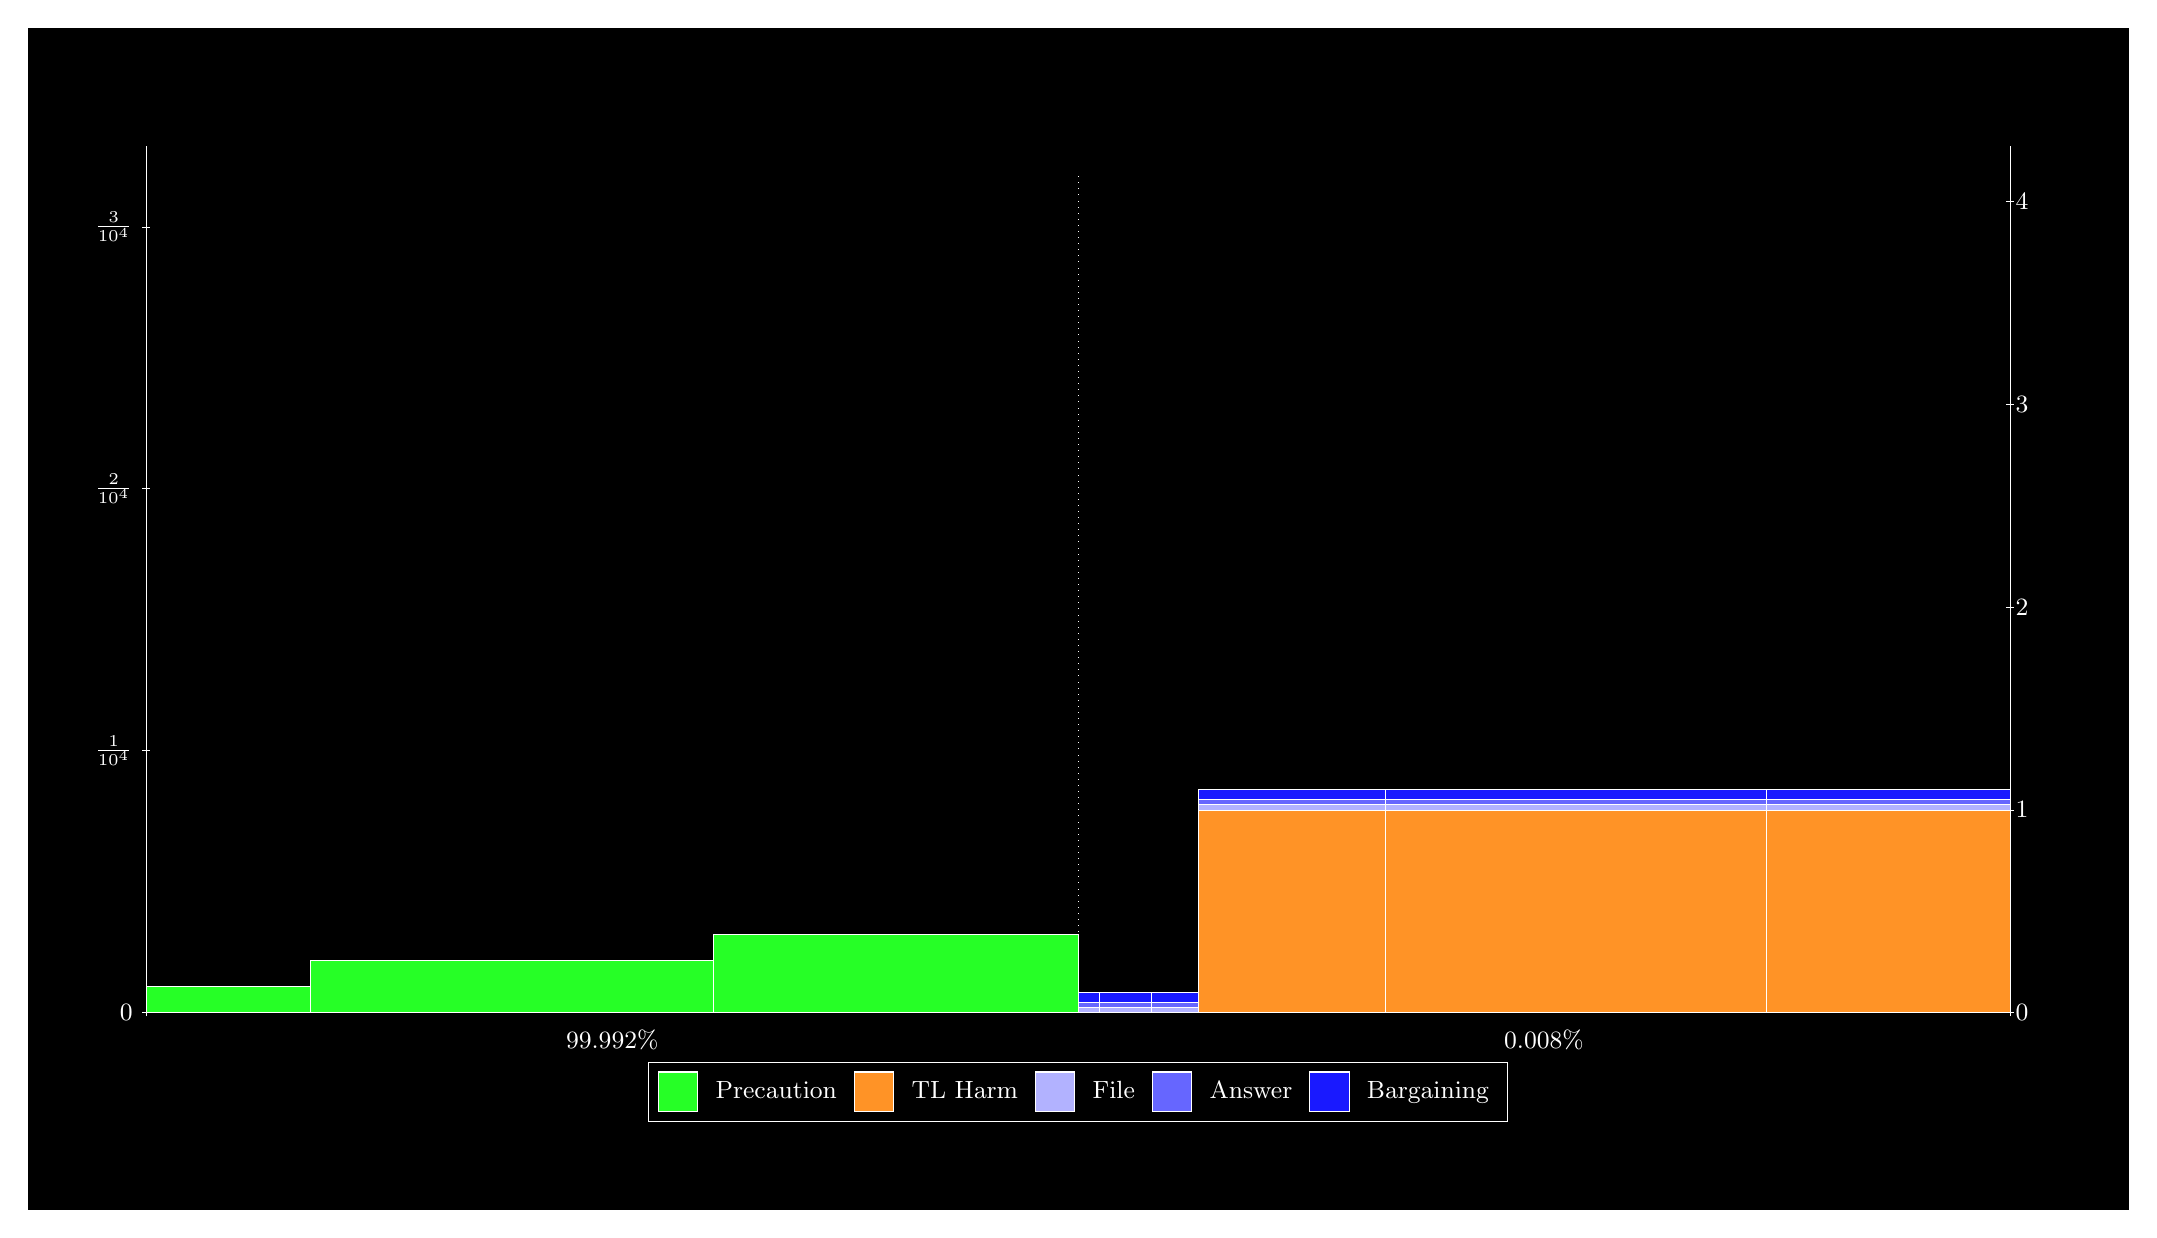
\begin{tikzpicture}
\draw[fill=black] (0,0) rectangle (26.667,15);
\draw[fill=green!85,draw=white,very thin] (1.5,2.5) rectangle (3.585,2.8326);
\draw[fill=green!85,draw=white,very thin] (3.585,2.5) rectangle (8.696,3.1652);
\draw[fill=green!85,draw=white,very thin] (8.696,2.5) rectangle (13.333,3.4977);
\draw[fill=green!85,draw=white,very thin] (13.333,2.5) rectangle (13.603,2.5);
\draw[fill=blue!30,draw=white,very thin] (13.333,2.5) rectangle (13.603,2.5644);
\draw[fill=blue!60,draw=white,very thin] (13.333,2.5644) rectangle (13.603,2.6287);
\draw[fill=blue!90,draw=white,very thin] (13.333,2.6287) rectangle (13.603,2.7574);
\draw[fill=green!85,draw=white,very thin] (13.603,2.5) rectangle (14.263,2.5001);
\draw[fill=blue!30,draw=white,very thin] (13.603,2.5001) rectangle (14.263,2.5644);
\draw[fill=blue!60,draw=white,very thin] (13.603,2.5644) rectangle (14.263,2.6287);
\draw[fill=blue!90,draw=white,very thin] (13.603,2.6287) rectangle (14.263,2.7574);
\draw[fill=green!85,draw=white,very thin] (14.263,2.5) rectangle (14.862,2.5001);
\draw[fill=blue!30,draw=white,very thin] (14.263,2.5001) rectangle (14.862,2.5644);
\draw[fill=blue!60,draw=white,very thin] (14.263,2.5644) rectangle (14.862,2.6288);
\draw[fill=blue!90,draw=white,very thin] (14.263,2.6288) rectangle (14.862,2.7575);
\draw[fill=green!85,draw=white,very thin] (14.862,2.5) rectangle (17.239,2.5);
\draw[fill=orange!85,draw=white,very thin] (14.862,2.5) rectangle (17.239,5.074);
\draw[fill=blue!30,draw=white,very thin] (14.862,5.074) rectangle (17.239,5.1383);
\draw[fill=blue!60,draw=white,very thin] (14.862,5.1383) rectangle (17.239,5.2027);
\draw[fill=blue!90,draw=white,very thin] (14.862,5.2027) rectangle (17.239,5.3314);
\draw[fill=green!85,draw=white,very thin] (17.239,2.5) rectangle (22.069,2.5001);
\draw[fill=orange!85,draw=white,very thin] (17.239,2.5001) rectangle (22.069,5.074);
\draw[fill=blue!30,draw=white,very thin] (17.239,5.074) rectangle (22.069,5.1384);
\draw[fill=blue!60,draw=white,very thin] (17.239,5.1384) rectangle (22.069,5.2027);
\draw[fill=blue!90,draw=white,very thin] (17.239,5.2027) rectangle (22.069,5.3314);
\draw[fill=green!85,draw=white,very thin] (22.069,2.5) rectangle (25.167,2.5001);
\draw[fill=orange!85,draw=white,very thin] (22.069,2.5001) rectangle (25.167,5.074);
\draw[fill=blue!30,draw=white,very thin] (22.069,5.074) rectangle (25.167,5.1384);
\draw[fill=blue!60,draw=white,very thin] (22.069,5.1384) rectangle (25.167,5.2027);
\draw[fill=blue!90,draw=white,very thin] (22.069,5.2027) rectangle (25.167,5.3314);
\draw[white,very thin] (1.5,2.5) -- (1.5,13.5);
\draw[white,very thin] (1.45,2.5) -- (1.55,2.5);
\node[font=\small,text=white, anchor=east] at (1.45, 2.5) {0};
\draw[white,very thin] (1.45,5.8258) -- (1.55,5.8258);
\node[font=\small,text=white, anchor=east] at (1.45, 5.8258) {$\frac{1}{10^{4}}$};
\draw[white,very thin] (1.45,9.1516) -- (1.55,9.1516);
\node[font=\small,text=white, anchor=east] at (1.45, 9.1516) {$\frac{2}{10^{4}}$};
\draw[white,very thin] (1.45,12.477) -- (1.55,12.477);
\node[font=\small,text=white, anchor=east] at (1.45, 12.477) {$\frac{3}{10^{4}}$};

\draw[white,dotted,very thin] (13.333,2.83) -- (13.333,13.17);
\draw[white,very thin] (25.167,2.5) -- (25.167,13.5);
\draw[white,very thin] (25.117,2.5) -- (25.217,2.5);
\node[font=\small,text=white, anchor=west] at (25.117, 2.5) {0};
\draw[white,very thin] (25.117,5.074) -- (25.217,5.074);
\node[font=\small,text=white, anchor=west] at (25.117, 5.074) {1};
\draw[white,very thin] (25.117,7.6479) -- (25.217,7.6479);
\node[font=\small,text=white, anchor=west] at (25.117, 7.6479) {2};
\draw[white,very thin] (25.117,10.222) -- (25.217,10.222);
\node[font=\small,text=white, anchor=west] at (25.117, 10.222) {3};
\draw[white,very thin] (25.117,12.796) -- (25.217,12.796);
\node[font=\small,text=white, anchor=west] at (25.117, 12.796) {4};

\draw[white,very thin] (1.5,2.5) -- (25.167,2.5);
\draw[white,very thin] (1.5,2.45) -- (1.5,2.55);
\node[font=\small,text=white, anchor=north] at (1.5, 2.45) {};
\draw[white,very thin] (25.167,2.45) -- (25.167,2.55);
\node[font=\small,text=white, anchor=north] at (25.167, 2.45) {};

\node[font=\small,text=white,anchor=south] at (7.4167, 1.9) {99.992\%};
\node[font=\small,text=white,anchor=south] at (19.25, 1.9) {0.008\%};
\draw (13.3333,2.5) node (B) {};
\begin{scope}[align=center]
\matrix[scale=0.5,draw=white,below=0.5cm of B,nodes={draw},column sep=0.1cm]{
\node[rectangle,draw,minimum width=0.5cm,minimum height=0.5cm,fill=green!85]{}; & \node[draw=none,font=\small,text=white]{Precaution}; &
\node[rectangle,draw,minimum width=0.5cm,minimum height=0.5cm,fill=orange!85]{}; & \node[draw=none,font=\small,text=white]{TL Harm}; &
\node[rectangle,draw,minimum width=0.5cm,minimum height=0.5cm,fill=blue!30]{}; & \node[draw=none,font=\small,text=white]{File}; &
\node[rectangle,draw,minimum width=0.5cm,minimum height=0.5cm,fill=blue!60]{}; & \node[draw=none,font=\small,text=white]{Answer}; &
\node[rectangle,draw,minimum width=0.5cm,minimum height=0.5cm,fill=blue!90]{}; & \node[draw=none,font=\small,text=white]{Bargaining}; \\\\
};\end{scope}

\end{tikzpicture}
\end{document}